\documentclass[a4paper,ngerman,12pt]{scrartcl}

\usepackage[utf8]{inputenc}

\usepackage[ngerman]{babel}

\usepackage{amsmath,amsthm,amssymb,stmaryrd,color,graphicx,mathtools}
\usepackage{array}
\usepackage{xstring}

\usepackage[protrusion=true,expansion=true]{microtype}

\usepackage{lmodern}
\usepackage{tabto}

\usepackage[all]{xy}

\usepackage{tikz}
\usetikzlibrary{calc,shapes.callouts,shapes.arrows}
\newcommand{\hcancel}[5]{%
    \tikz[baseline=(tocancel.base)]{
        \node[inner sep=0pt,outer sep=0pt] (tocancel) {#1};
        \draw[red, line width=0.5mm] ($(tocancel.south west)+(#2,#3)$) -- ($(tocancel.north east)+(#4,#5)$);
    }%
}

\usepackage{hyperref}

\theoremstyle{definition}
\newtheorem{defn}{Definition}[section]
\newtheorem{bsp}[defn]{Beispiel}

\theoremstyle{plain}

\newtheorem{prop}[defn]{Proposition}
\newtheorem{lemma}[defn]{Lemma}
\newtheorem{satz}[defn]{Satz}

\theoremstyle{remark}
\newtheorem{bem}[defn]{Bemerkung}

\clubpenalty=10000
\widowpenalty=10000
\displaywidowpenalty=10000

\setlength\parskip{\medskipamount}
\setlength\parindent{0pt}

\newcommand{\NN}{\mathbb{N}}
\newcommand{\ZZ}{\mathbb{Z}}
\renewcommand{\aa}{\mathfrak{a}}
\newcommand{\bb}{\mathfrak{b}}
\newcommand{\pp}{\mathfrak{p}}
\renewcommand{\O}{\mathcal{O}}
\DeclareMathOperator{\Spec}{Spec}
\renewcommand{\_}{\mathpunct{.}\,}
\newcommand{\?}{\,{:}\,}
\newcommand{\defeq}{\vcentcolon=}

\newcommand{\hilight}[2]{\begin{center}\framebox{#2}\par#1\end{center}}

\newcommand{\speak}[1]{\ulcorner\text{#1}\urcorner}

\renewcommand*\theenumi{\alph{enumi}}
\renewcommand{\labelenumi}{\theenumi)}

\setcounter{tocdepth}{2}

\newlength{\aufgabenskip}
\setlength{\aufgabenskip}{1.5em}
\newcounter{aufgabennummer}
\newenvironment{aufgabe}[1]{
  \addtocounter{aufgabennummer}{1}
  \textbf{Aufgabe \theaufgabennummer{}.} \emph{#1} \par
}{\vspace{\aufgabenskip}}

\newenvironment{indentblock}{%
  \list{}{\leftmargin\leftmargin}%
  \item\relax
}{%
  \endlist
}

\newif\ifklein\kleinfalse
\IfSubStr{\jobname}{\detokenize{klein}}{\kleintrue}{\kleinfalse}

\begin{document}

\title{Spiel und Spaß mit der internen Welt des kleinen Zariski-Topos}
\author{Ingo Blechschmidt}
\date{23. Dezember 2015}
\maketitle

\thispagestyle{empty}
\enlargethispage{3cm}
\begin{center}
  \ifklein
    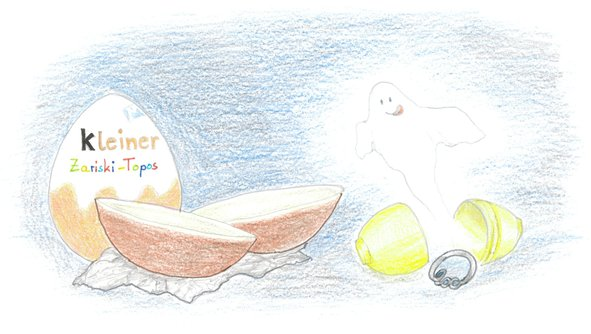
\includegraphics[scale=3]{zariski-ueberraschung-klein.jpeg}
  \else
    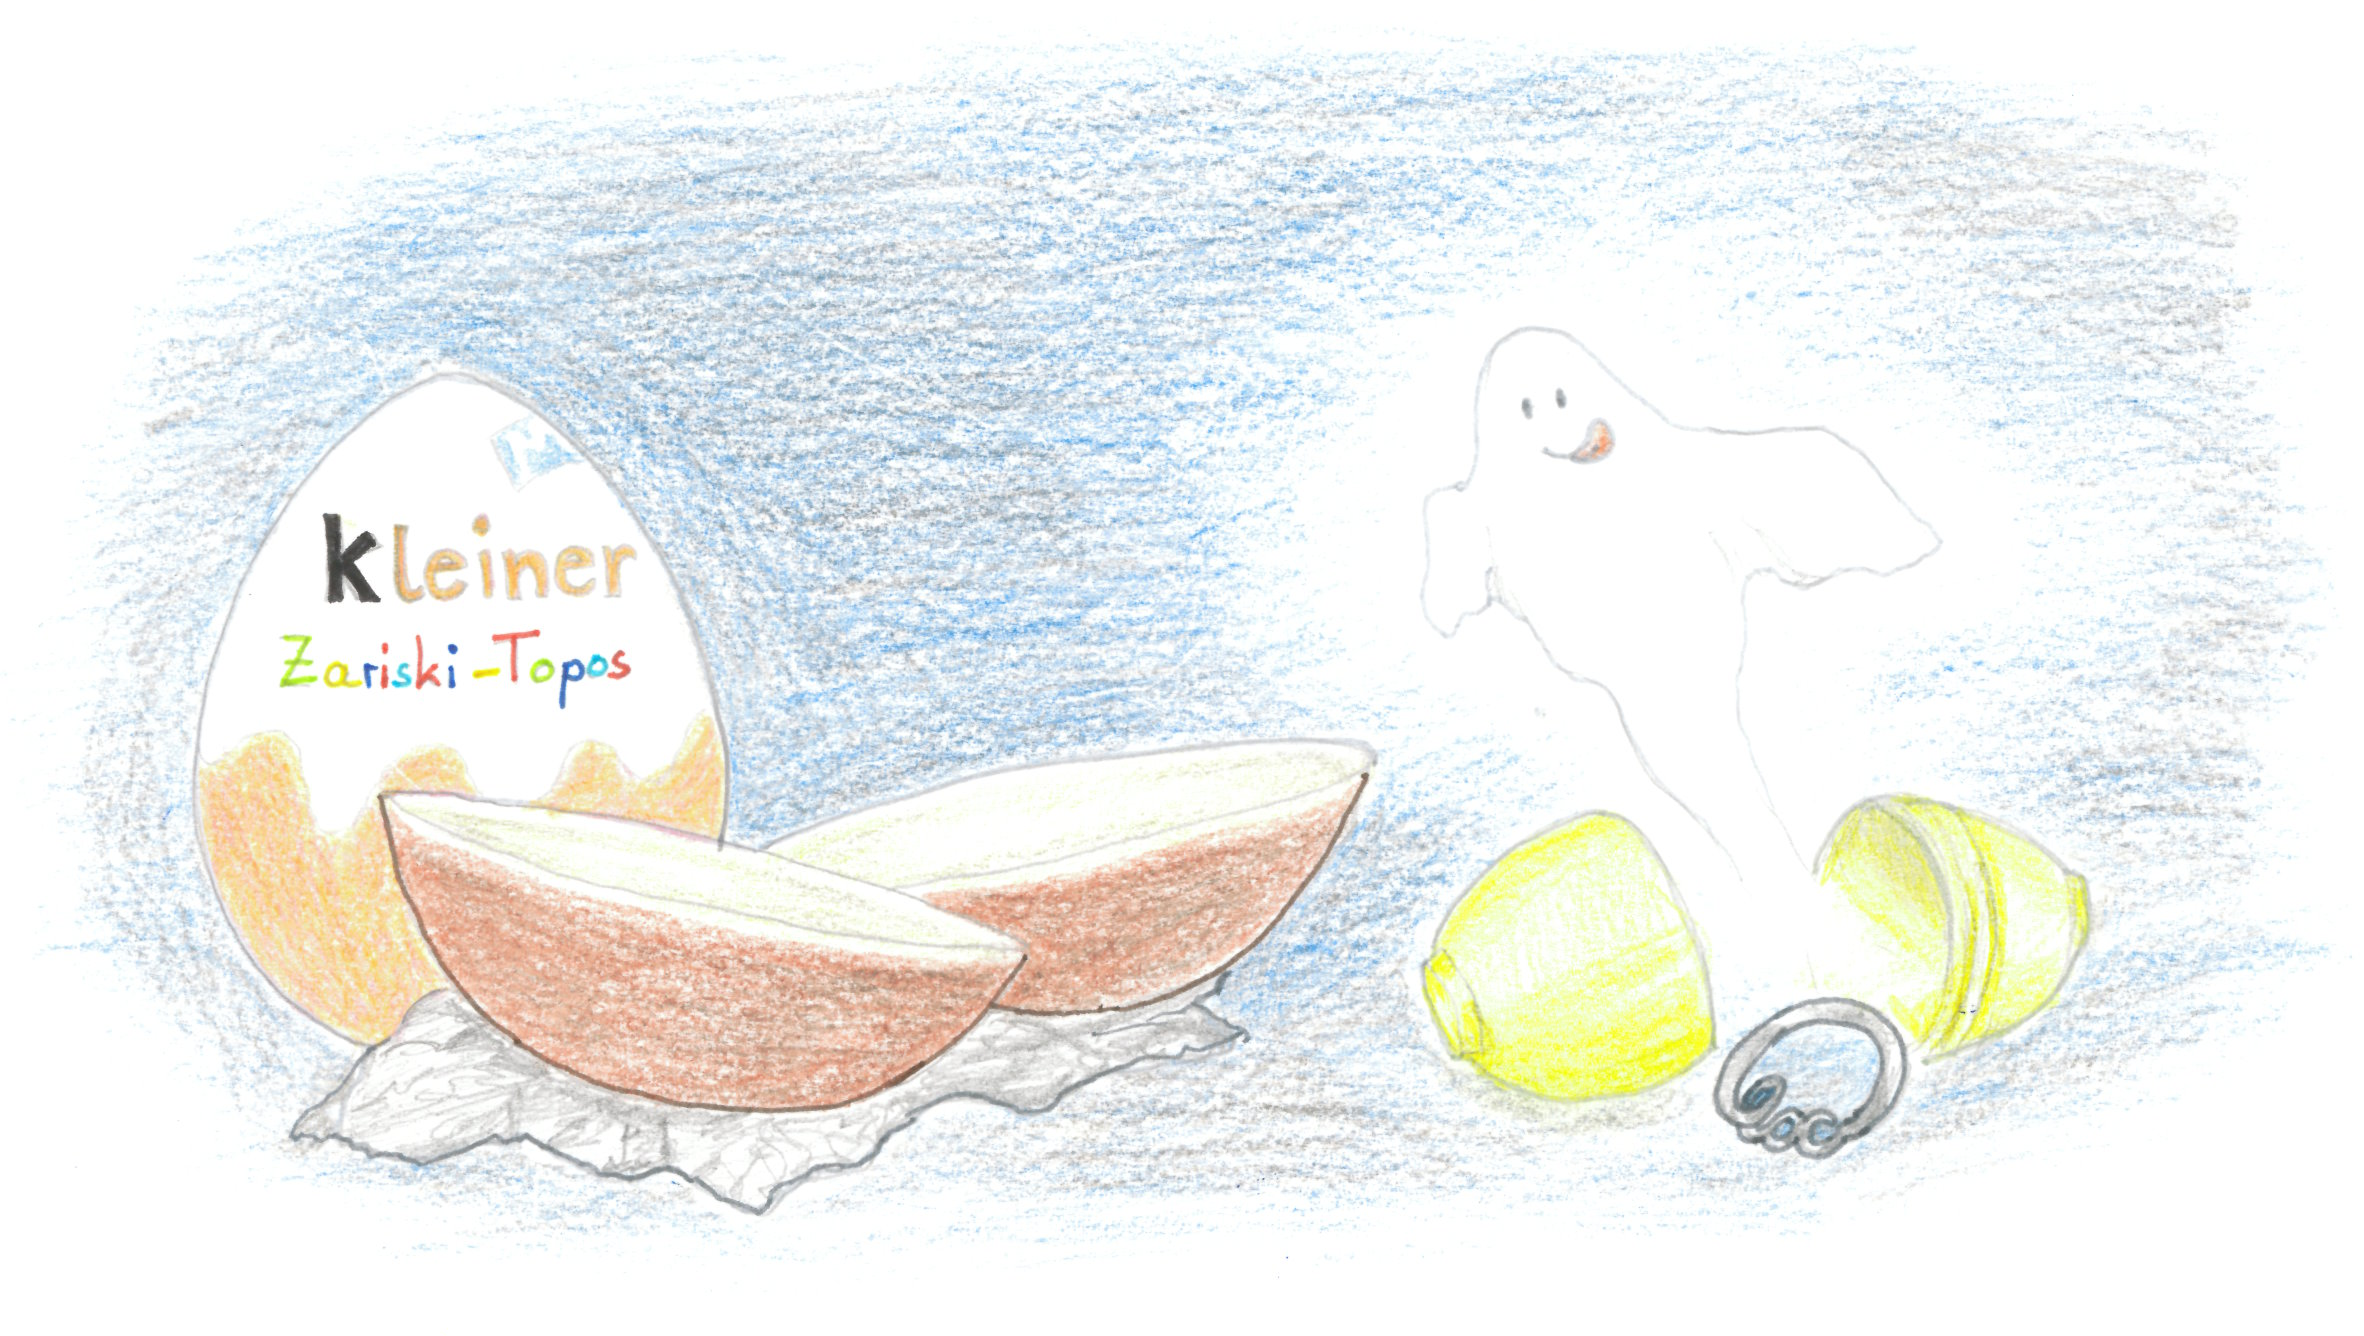
\includegraphics[scale=0.75]{zariski-ueberraschung}
  \fi
\end{center}
\vfill
\newcommand{\Ll}{:\Longleftrightarrow}
\hilight{Die Kripke--Joyal-Semantik des kleinen Zariski-Topos.}{%
  $\renewcommand{\arraystretch}{1.3}\begin{array}{@{}lcl@{}}
    R \models x = y \? \O &\Ll&
      \text{Für die gegebenen Elemente $x, y \in R$ gilt $x = y$.} \\
    R \models \top &\Ll&
      1 = 1 \in R. \text{ (Das ist stets erfüllt.)} \\
    R \models \bot &\Ll&
      1 = 0 \in R. \text{ (Das ist genau in Nullringen erfüllt.)} \\
    R \models \phi \wedge \psi &\Ll&
      \text{$R \models \phi$ und $R \models \psi$.} \\
    R \models \phi \vee \psi &\Ll&
      \hcancel{\text{$R \models \phi$ oder $R \models \psi$.}}{0pt}{3pt}{0pt}{-2pt} \\
    R \models \phi \vee \psi &\Ll&
      \text{Es gibt eine Zerlegung $\sum_i s_i = 1 \in R$ sodass} \\
    &&{\quad\quad} \text{für alle~$i$ jeweils $R[s_i^{-1}] \models \phi$
      oder $R[s_i^{-1}] \models \psi$.} \\
    R \models \phi \Rightarrow \psi &\Ll&
      \text{Für jedes~$s \in R$ gilt: Aus $R[s^{-1}] \models \phi$ folgt $R[s^{-1}] \models \psi$.} \\
    R \models \forall x\?\O\_ \phi &\Ll&
      \text{Für jedes~$s \in R$ und jedes $x \in R[s^{-1}]$
      gilt: $R[s^{-1}] \models \phi(x)$.} \\
    R \models \exists x\?\O\_ \phi &\Ll&
      \text{Es gibt eine Zerlegung $\sum_i s_i = 1 \in R$ und} \\
    &&{\quad\quad} \text{Elemente $x_i \in R[s_i^{-1}]$ sodass für alle $i$:
    $R[s_i^{-1}] \models \phi(x_i)$.}
  \end{array}$%
}

\newpage

\section*{Zusammenfassung}
%\begin{center}\begin{minipage}{0.8\textwidth}
Neben der üblichen mathematischen Welt gibt es alternative mathematische
Universen, sog. \emph{Topoi}. In diesen gelten leicht andere Gesetze der Logik.
Speziell gibt es zu jedem kommutativen Ring seinen zugehörigen \emph{kleinen
Zariski-Topos}, der darauf zugeschnitten ist, um \emph{lokal} über den Ring zu
sprechen. In diesen informalen Notizen wollen wir verstehen, wie man in diesem
alternativen Universum arbeiten kann.
%\end{minipage}\end{center}

Illustrationen: Carina Willbold

\tableofcontents

\newpage

\section{Vorbereitungen}

\subsection{Etwas formale Logik}

Im Folgenden wollen wir über mathematische Aussagen sprechen, in denen
\[ {=} \quad {\top} \quad {\bot} \quad {\wedge} \quad {\vee} \quad {\Rightarrow} \quad {\forall} \quad {\exists} \]
die einzigen vorkommenden logischen Symbole sind. Dabei steht~"`$\bot$"' für
eine ausgezeichnete falsche und~"`$\top$"' für eine ausgezeichnete wahre Aussage.
Negation ist ebenfalls wichtig, muss aber nicht als primitiv
angenommen werden, da man sie über die Beziehung
\[ \neg\phi \quad:\equiv\quad (\phi \Rightarrow \bot) \]
durch~$\Rightarrow$ und~$\bot$ ausdrücken kann: Zu behaupten, dass~$\phi$ nicht
stimmt, ist gleichbedeutend damit, zu behaupten, dass aus der Annahme
von~$\phi$ ein Widerspruch folgt.
Wir schreiben die universelle und existenzielle Quantifikation nicht mit dem
Elementsymbol, sondern dem in der Typtheorie üblichen Doppelpunkt:
\[ \forall x\?X\_ \phi(x). \]
Gelegentlich werden wir die Abhängigkeit von~$\phi(x)$ von~$x$ in der Notation
unterdrücken und kurz nur~"`$\phi$"' schreiben. Ferner verwenden wir den
Quantor der eindeutigen Existenz, formal definiert als
\[ \exists! x\?X\_ \phi(x) \quad:\equiv\quad
  \bigl(\exists x\?X\_ \phi(x)\bigr) \ \wedge\ \bigl(\forall x\?X\_ \forall x'\?X\_
  (\phi(x) \wedge \phi(x') \Rightarrow x = x')\bigr). \]
%Da wir (gezwungenermaßen) in einem konstruktiven Kontext arbeiten werden,
%können wir im Wesentlichen keine weiteren der aufgeführten primitiven Symbole
%durch die anderen ausdrücken. Etwa können wir \emph{nicht} die Regel
%\[ \phi \vee \psi \quad\Longleftrightarrow\quad \neg(\neg\phi \wedge \neg\psi) \]
%verwenden, um Disjunktion auf Negation und Konjunktion zurückzuführen -- die
%umgangssprachliche Interpretation der Aussage auf der linken Seite ist, dass
%wir wissen, dass~$\phi$ gilt oder dass~$\psi$ gilt, während in der rechten
%Aussage nur die Information steckt, dass es nicht sein kann, dass~$\phi$
%und~$\psi$ beide falsch sind.


\subsection{Geometrische Vorstellung von Ringen}

Zu einem kommutativen Ring~$R$ können wir uns einen geometrischen Raum~$\Spec
R$ vorstellen, und zwar auf solche Art und Weise, dass ein
Ringelement~$s \in R$ einer "`guten"' Funktion auf~$\Spec R$ entspricht.
Den Ort, wo diese Funktion nicht verschwindet, wollen wir mit~"`$D(s)$"'
bezeichnen. Dieser Ort ist stets eine offene Menge.

\begin{bsp}Den Ring~$K[X,Y]$ stellen wir uns geometrisch als~$K^2$ vor. Zum
Element~$s \defeq 2X+3Y$ gehört dann die Funktion~$(x,y) \mapsto 2x+3y$. Die
Menge~$D(s)$ ist das Komplement einer schrägen Gerade in~$K^2$.\end{bsp}

In diesem Bild können wir uns eine Zerlegung~$1 = \sum_i s_i \in R$ der Eins
als eine Über\-de\-ckung~$\bigcup_i D(s_i)$ von~$\Spec R$ vorstellen: Da die
Einsfunktion nirgendwo Null ist, können an keinem Punkt alle~$s_i$ zugleich
verschwinden.


\section{Die Kripke--Joyal-Semantik des kleinen Zariski-Topos}

Zu jedem kommutativen Ring~$R$ gehört ein alternatives Mathematik-Universum,
der \emph{kleine Zariski-Topos zu~$R$}. Uns fehlen kategorientheoretische
Konzepte, um dieses Universum explizit anzugeben (obwohl das nicht intrinsisch
schwer ist). Wir können aber beschreiben, was es bedeuten soll, dass \emph{eine
Aussage~$\phi$ in dem kleinen Zariski-Topos zu~$R$ gilt}, in Formeln
ausgedrückt als
\[ R \models \phi. \]

\begin{defn}Die Bedeutung von Aussagen der \emph{internen Sprache des
Zariski-Topos} soll durch Rekursion über den Aussageaufbau durch die auf der
ersten Seite angegebenen Übersetzungsregeln festgelegt sein.\end{defn}

Auf den ersten Blick erscheinen diese Regeln völlig
willkürlich. Tatsächlich aber sind sie fein aufeinander abgestimmt, schon
kleine Änderungen führen dazu, dass das gesamte System zusammenbricht. In
diesem Rahmen wollen wir sie schlichtweg als gegeben hinnehmen. Durch die
Beispiele im folgenden Abschnitt werden wir uns schnell an sie gewöhnen.

In dem kleinen Zariski-Topos zu~$R$ gibt es ein Abbild des Rings~$R$, das
wir~"`$\O$"' schreiben. (Diese Bezeichnung hat nichts mit Ganzheitsringen zu tun.)


\section{Erste Gehversuche in der internen Welt}

\subsection{Interne Kommutativität}

Mit den Übersetzungsregeln an der Hand können wir beginnen, die interne Welt zu
erkunden. Folgende Beobachtung macht den Anfang:

\begin{prop}Der Ring~$\O$ des kleinen Zariski-Topos zu~$R$ ist wieder
kommutativ -- das heißt:
\[ R \models \forall x,y \? \O\_ x y = y x. \]
\end{prop}
\begin{proof}Die Doppelquantifikation in der Behauptung ist eine
Kurzschreibweise für
\[ R \models \forall x\?\O\_ \forall y\?\O\_ x y = y x. \]
Gemäß den Regeln bedeutet das:
\begin{indentblock}
Für alle~$s \in R$ und alle~$x \in R[s^{-1}]$ gilt:
\begin{indentblock}
Für alle~$t \in R[s^{-1}]$ und alle~$y \in R[s^{-1}][t^{-1}]$ gilt:
\begin{indentblock}
In~$R[s^{-1}][t^{-1}]$ gilt~$xy = yx$.
\end{indentblock}
\end{indentblock}
\end{indentblock}
Das erscheint vielleicht etwas verklausuliert, ist aber auch offensichtlich
wahr.
\end{proof}


\subsection{Interne Invertierbarkeit}

Das folgende Lemma ist ähnlich. Es besagt, dass es keinen Unterschied zwischen
Invertierbarkeit aus interner und externer (also üblicher) Sicht gibt.
\begin{prop}\label{interne-invertierbarkeit}%
Genau dann ist ein Ringelement~$f \in R$ invertierbar, wenn es als Element
von~$\O$ invertierbar ist, wenn also
\[ R \models \exists g\?\O\_ fg = 1. \]
\end{prop}
\begin{proof}
Die Übersetzung der internen Aussage lautet:
\begin{indentblock}
Es gibt eine Zerlegung~$1 = \sum_i s_i \in R$, sodass für jeden Index~$i$ ein
Element $g_i \in R[s_i^{-1}]$ mit~$fg_i = 1$ in~$R[s_i^{-1}]$ existiert.
\end{indentblock}
Damit ist es nur noch eine Übungsaufgabe in elementarer Ringtheorie, die
behauptete Äquivalenz nachzuweisen.
\end{proof}


\subsection{Interne Lokalität}

Diese beiden Propositionen waren noch nicht besonders beeindruckend.
Die folgende Proposition ist dagegen beim ersten Kontakt völlig verblüffend und
illustriert gut den kuriosen Charakter der internen Welt. Dazu erinnern wir an
das Konzept eines lokalen Rings:
\begin{defn}Ein Ring heißt genau dann \emph{lokal}, wenn, wann immer eine Summe
von Ringelementen invertierbar ist, schon mindestens ein Summand invertierbar
ist.\end{defn}
\begin{bsp}Die vertrauten Ringe~$\ZZ$ und~$K[X,Y]$ sind nicht lokal. Oft erhält
man lokale Ringe durch geeignete Lokalisierung: Jeder Körper ist lokal,
die Lokalisierung~$\ZZ_{(p)}$ nach einem Primideal~$(p)$ ist lokal, der Ring
$K[X,Y]_{(X-a,Y-b)} = \{ f/g \,|\, f,g \in K[X,Y], g(a,b) \neq 0 \}$ der in
beliebig kleinen Umgebungen von~$(a,b) \in K^2$ definierten rationalen
Funktionen ist lokal.
\end{bsp}

\begin{bem}Die Namensgebung erklärt sich durch folgende Beobachtung: Ein
lokaler Ring~$R$ ist ein solcher, sodass jede offene Überdeckung von~$\Spec R$
schon eine einelementige Teilüberdeckung besitzt.\end{bem}

\begin{prop}\label{intern-lokal}%
Unabhängig davon, ob~$R$ lokal ist oder nicht, ist der Ring~$\O$
der internen Zariski-Welt stets lokal.\end{prop}
\begin{proof}
Wir zeigen, dass
\[ R \models \forall x,y\?\O\_\ \speak{$x+y$ inv.}\ \Longrightarrow\ 
  \speak{$x$ inv.} \,\vee\, \speak{$y$ inv.}. \]
Die Häkchen sollen andeuten, dass der entsprechende Teil nur umgangssprachlich
vorliegt und daher von der Leserin formalisiert werden muss. Unter Verwendung von
Proposition~\ref{interne-invertierbarkeit} (angewendet auf~$R'$
statt~$R$) weisen uns die
Übersetzungsregeln also an, folgende Behauptung zu zeigen:
\begin{indentblock}
Für alle~$s \in R$ und~$x \in R[s^{-1}]$ gilt:
\begin{indentblock}
Für alle~$t \in R[s^{-1}]$ und~$y \in R[s^{-1}][t^{-1}]$ gilt:
\begin{indentblock}
Für alle~$u \in R[s^{-1}][t^{-1}]$ gilt: Falls~$x+y$ in~$R[s^{-1}][t^{-1}][u^{-1}] =: R'$
invertierbar ist, so gibt es eine Zerlegung der Eins von~$R'$, $1 = v_1 +
\cdots + v_n \in R'$, sodass in den
weiter lokalisierten Ringen~$R'[v_i^{-1}]$ jeweils~$x$ oder~$y$ invertierbar
ist.
\end{indentblock}
\end{indentblock}
\end{indentblock}
Der Nachweis dieser Behauptung ist eine Übungsaufgabe.
\end{proof}

Mit der internen Welt des kleinen Zariski-Topos kann man also jeden
beliebigen Ring als einen lokalen Ring auffassen.


\section{Vereinfachungsregeln}

In den bisherigen Beispielen waren die übersetzten Aussagen
von recht verschachtelter Form. Bevor wir fortfahren, wollen wir daher
Vereinfachungsregeln festhalten, die den praktischen Umgang mit internen
Aussagen angenehmer gestalten.

\begin{lemma}\label{vereinfachung}%
Für folgende Quantorenfiguren kann man die Regeln vereinfachen:
\[\renewcommand{\arraystretch}{1.3}\begin{array}{@{}lcl@{}}
  R \models \forall x\?\O\_ \forall y\?\O\_ \phi &\Ll&
    \text{Für alle~$s \in R$ und~$x,y \in R[s^{-1}]$ gilt~$R[s^{-1}] \models
    \phi(x,y)$.} \\
  R \models \forall x\?\O\_ \phi \Rightarrow \psi &\Ll&
    \text{Für alle~$s \in R$ und~$x \in R[s^{-1}]$ gilt:} \\
  &&{\quad\quad} \text{Aus $R[s^{-1}] \models \phi(x)$ folgt $R[s^{-1}] \models \psi(x)$.} \\
  R \models \exists x\?\O\_ \exists y\?\O\_ \phi &\Ll&
    \text{Es gibt eine Zerlegung~$1 = \sum_i s_i \in R$ und} \\
  &&{\quad\quad} \text{für jeden Index~$i$ Elemente~$x_i, y_i \in R[s_i^{-1}]$} \\
  &&{\quad\quad} \text{mit $R[s_i^{-1}] \models \phi(x_i,y_i)$.} \\
  R \models \exists!x \? \O\_ \phi &\Ll&
    \text{Für alle~$s \in R$ existiert genau ein~$x \in R[s^{-1}]$ mit} \\
  &&{\quad\quad} R[s^{-1}] \models \phi(x). \\
  R \models \forall x\?\O\_ \exists! y\?\O\_ \phi &\Ll&
    \text{Für alle~$s \in R$ und~$x \in R[s^{-1}]$ existiert} \\
  &&{\quad\quad} \text{genau ein~$y \in R[s^{-1}]$ mit $R[s^{-1}] \models
  \phi(x,y)$.}
\end{array}\]
\end{lemma}
\begin{proof}Sobald man die internen Aussagen übersetzt hat, muss man nur ein
paar allgemeine Fakten über die Lokalisierung von Ringen nachweisen. Das ist
nicht schwer, aber auch nicht besonders erhellend.\end{proof}


\section{Fundamentale Eigenschaften der internen Sprache}

\subsection{Lokalität der internen Sprache}

In einem gewissen Sinn gilt~$R \models \phi$ genau dann, wenn~$\phi$ auf ganz~$\Spec R$
gilt. Dagegen bedeutet~$R[s^{-1}] \models \phi$ nur, dass~$\phi$ auf~$D(s)$
gilt.

Die interne Welt des kleinen Zariski-Topos zu~$R$ fasst nun gewissermaßen die
\emph{lokalen Aspekte} von~$R$ -- solche, die genau dann ganz~$\Spec R$
betreffen, wenn sie die einzelnen Überdeckungsmengen einer offenen
Überdeckung betreffen. Die folgende Proposition macht dieses Motto präzise:
\begin{prop}Sei~$1 = \sum_i s_i \in R$ eine Zerlegung der Eins und~$\phi$ eine
Aussage. Dann gilt genau dann~$R \models \phi$, wenn für alle~$i$
jeweils~$R[s_i^{-1}] \models \phi$ gilt.\end{prop}
\begin{proof}Induktion über den Aufbau von~$\phi$.\end{proof}

Eine Aussage~$\phi$ muss also nicht unbedingt im Wortlaut erfüllt sein, um in
der internen Welt des kleinen Zariski-Topos zu gelten. Es genügt, dass es
eine Zerlegung der Eins gibt, sodass sie in den jeweils lokalisierten Ringen gilt.
Die technische Verwaltung der Zerlegungen übernimmt dabei der
Übersetzungsapparat; mit der internen Welt ist es also möglich, \emph{lokal}
mit Ringen zu arbeiten, ohne manuell Zerlegungen einführen und mitschleppen
zu müssen.

\begin{bsp}\label{lokal-hauptideale}%
Sei~$R$ ein prüferscher Bereich, also ein Integritätsbereich, in dem jedes endlich erzeugtes
Ideal~$\aa$ \emph{lokal} ein
Hauptideal ist -- in dem Sinn, dass es eine Zerlegung~$1 = \sum_i s_i$ der Eins
gibt, sodass die erweiterten Ideale~$\aa[s_i^{-1}]$ jeweils in~$R[s_i^{-1}]$
Hauptideale sind. Der Ring~$\O$ der internen Welt spiegelt diese Eigenschaft
viel einfacher wieder: Er ist \emph{bézoutsch} -- jedes endlich
erzeugte Ideal ist selbst schon ein Hauptideal.\end{bsp}


\subsection{Verträglichkeit mit konstruktiver Logik}

Bisher haben wir die interne Welt des kleinen Zariski-Topos allein dadurch
erkundet, indem wir mit den Kripke--Joyal-Regeln die Rückübersetzung in unsere
gewohnte mathematische Sprache vorgenommen haben. Wenn das unsere einzige
Interaktionsmöglichkeit mit der internen Welt wäre, wäre das ganze Thema nicht
besonders spannend. Tatsächlich aber können wir in der internen Welt auch
\emph{mathematisch argumentieren} -- fast genau so, wie wir es gewohnt sind.

\begin{satz}\label{soundness}%
Wenn~$R \models \phi$ gilt und konstruktiv aus~$\phi$ eine weitere
Aussage~$\psi$ folgt, so gilt auch~$R \models \psi$.\end{satz}
\begin{proof}Wir müssen uns
zunächst überlegen, aus welchen grundlegenden Argumentationsschritten Beweise
aufgebaut sind. Dann müssen wir von jedem solchen Baustein nachweisen,
dass er in der internen Welt ebenfalls erfüllt ist. Etwa gibt es das logische
Prinzip
\begin{indentblock}\emph{Wenn $\phi \wedge \psi$ gilt, so gilt auch~$\phi$}.
\end{indentblock}
Dieses ist in der internen Sprache ebenfalls erfüllt, denn aus~$R \models \phi
\wedge \psi$ folgt nach den Übersetzungsregeln sofort~$R \models \phi$.

Die Hauptschwierigkeit eines präzisen Beweises des Satzes liegt darin,
eine über\-sicht\-li\-che Liste von Kernbeweisschritten derart zusammenzustellen,
dass jede denkbare Argumentation so formalisiert werden kann, dass sie nur diese
Bausteine verwendet. Danach ist es nur noch ein einfacher Induktionsbeweis über den
Aufbau formal niedergeschriebener konstruktiver Beweise.
\end{proof}

\begin{bsp}Man kann konstruktiv zeigen, dass jede Matrix über einem lokalen
Ring, die einen Rang besitzt, mittels elementarer Zeilen- und Spaltentransformationen auf eine
Diagonalgestalt gebracht werden kann. Daraus folgt \emph{ohne weiteres Zutun}
sofort, dass man jede Matrix (die einen Rang besitzt) über einem
\emph{beliebigen} Ring \emph{lokal} auf eine Diagonalgestalt bringen kann -- in dem Sinn, dass es
eine Zerlegung der Eins gibt, sodass in den lokalisierten Ringen die Matrix
jeweils äquivalent zu einer Diagonalmatrix ist: Denn nach Proposition~\ref{intern-lokal}
ist der Ring~$\O$ der internen Welt ja stets lokal.\end{bsp}

\begin{bem}Ein direkter Beweis der Behauptung über die Diagonalisierbarkeit
über beliebigen Ringen ist natürlich ebenfalls möglich. Er erfordert jedoch
die Einführung, Verwaltung und Kombination mehrerer Zerlegungen der Eins. Diese
technischen Schritte fallen bei Arbeit in der internen Welt ersatzlos weg. Um
Zerlegungen der Eins muss man sich nur ein einziges Mal kümmern, nämlich im
Beweis des allgemeinenen Satzes~\ref{soundness}.\end{bem}


\section{Der nichtklassische Charakter der internen Welt}

Satz~\ref{soundness} erlaubt es, über den Ring~$\O$ der internen Welt
wie üblich mathematisch zu argumentieren -- solange man dabei nur konstruktive
Logik verwendet, also sich \emph{nicht} auf die sonst üblichen Axiome
\begin{itemize}
\item \emph{Prinzip vom ausgeschlossenen Dritten:} $\phi \vee \neg\phi$
\item \emph{Prinzip der Doppelnegationselimination:} $\neg\neg\phi \Rightarrow
\phi$
\item \emph{Auswahlaxiom}
\end{itemize}
beruft. Das ist anfangs ungewohnt, bedeutet in Anwendungen der Mathematik aber
oftmals keine große Einschränkung.

Die Beschränkung auf konstruktive Logik ist dabei keine Frage der Einstellung
-- die interne Welt erfüllt nun mal nicht die genannten klassischen Axiome. Das
wollen wir in diesem Abschnitt einsehen.

\begin{lemma}Sei~$f \in R$. Genau dann ist~$f$ in der internen Welt nicht
invertierbar, wenn~$f$ im gewöhnlichen Sinn nilpotent ist.\end{lemma}
\begin{proof}Die Aussage~$R \models \neg(\speak{$f$ inv.})$ lautet ausgeschrieben
\[ R \models \bigl(\exists g\?\O\_ fg = 1\bigr) \Rightarrow \bot \]
und übersetzt sich unter Zuhilfenahme der Vereinfachungsregeln aus Lemma~\ref{vereinfachung}
und Lemma~\ref{interne-invertierbarkeit} wie folgt:
\begin{indentblock}
Für alle~$s \in R$ gilt:
\begin{indentblock}
Sollte~$f$ in~$R[s^{-1}]$ invertierbar sein, so gilt~$1 = 0$ in~$R[s^{-1}]$
(das ist gleichbedeutend damit, dass~$s$ nilpotent ist).
\end{indentblock}
\end{indentblock}
Durch die Spezialisierung~$s \defeq f$ erhalten wir daher sofort die Hinrichtung.
Wenn umgekehrt~$f$ nilpotent ist, enthalten die lokalisierten Ringe~$R[s^{-1}]$
ein invertierbares und trotzdem nilpotentes Element. Das geht nur, wenn sie
Nullringe sind.
\end{proof}

\begin{prop}In der internen Welt des kleinen Zariski-Topos eines Rings gilt im
Allgemeinen \emph{nicht}, dass jedes Element von~$\O$ invertierbar oder nicht
invertierbar ist. Insbesondere gilt im kleinen Zariski-Topos das Prinzip vom ausgeschlossenen Dritten
also \emph{nicht}.
\end{prop}
\begin{proof}Ein Gegenbeispiel liefert der Ring~$R \defeq \ZZ$ mit dem Element~$f
\defeq 2$. Denn
\[ R \models \speak{$f$ inv.} \vee \neg(\speak{$f$ inv.}) \]
bedeutet, dass es eine Zerlegung~$1 = s_1 + \cdots + s_n$ der Eins
von~$\ZZ$ gibt, sodass in den lokalisierten Ringen~$\ZZ[s_i^{-1}]$ die Zahl~$2$
jeweils invertierbar oder nilpotent ist. In einer solchen Zerlegung muss eine der Zahlen~$s_i$ ungerade
sein. In den Nennern der Elemente des zugehörigen lokalisierten
Rings~$\ZZ[s_i^{-1}]$ dürfen also gewisse ungerade Zahlen stehen (Potenzen
von~$s_i$). Daher ist die Zahl~$2$ dort weiterhin nicht invertierbar. Sie ist
aber auch nicht nilpotent.
\end{proof}


\section{Ausblick}

\subsection*{Weitere Objekte des kleinen Zariski-Topos}

Bisher haben wir nur über die Eigenschaften des Rings~$\O$ der internen Welt
des kleinen Zariski-Topos gesprochen. Genau wie in der üblichen mathematischen
Welt gibt es aber auch im Zariski-Topos noch viele weitere Objekte, etwa
den Polynomring~$\O[X]$ und den Matrizenringoid~$\amalg_{n,m} \O^{n \times
m}$ sowie Objekte, die nicht zur Ringtheorie gehören, wie
Analoga zu Potenzmengen.

Es ist leicht, die Regeln der Kripke--Joyal-Semantik so zu erweitern, dass man
auch über diese weiteren Objekte nativ sprechen kann. In der vollen internen
Sprache kann man sogar, wie im üblichen mathematischen Universum auch, aus
gegebenen Objekten über Operationen wie Potenzmengenbildung, Ausschneidung von
Teilmengen, Bildung von Faktormengen und so weiter neue konstruieren. Damit
steht die interne Sprache der üblichen mathematischen Sprache in keiner
Hinsicht nach -- bis auf die Einschränkung auf konstruktive Logik.


\subsection*{Verständnis für konstruktive Logik}

Wir haben gesehen, dass in der internen Welt des kleinen Zariski-Topos nur die
Gesetze konstruktiver Logik gelten. Möchten wir in der internen Welt
mathematisch argumentieren, haben wir also keine andere Wahl, als auf das
klassische Prinzip des ausgeschlossenen Dritten und verwandte Prinzipien zu
verzichten.

Es gibt eine Möglichkeit, diesen Verzicht auch ohne topostheoretischen
Hintergrund anschaulich zu deuten: Dass eine Aussage konstruktiv gilt, kann man
sich so vorstellen, dass man einen \emph{expliziten Beleg} für die Gültigkeit
der Aussage hat. Dann bedeutet eine zusammengesetzte Aussage
wie $\phi \vee \psi$,
dass man einen Beleg für~$\phi$ oder einen Beleg für~$\psi$ hat -- das ist
schwächer als die klassische Interpretation derselben Aussage, nach der~$\phi$
oder~$\psi$ lediglich wahr sind.

Die negierte Aussage
\[ \neg\phi \quad\equiv\quad (\phi \Rightarrow \bot) \]
bedeutet, dass man aus einem Beleg von~$\phi$ einen Beleg der falschen
Aussage~$\bot$ produzieren könnte. Da es einen solchen nicht gibt,
bedeutet~$\neg\phi$ also, dass es keinen Beleg für~$\phi$ gibt.
In diesem Bild besagt das Prinzip der Doppelnegationselimination,
\[ \neg\neg\phi \Longrightarrow \phi, \]
dass man, wenn man weiß, dass es nicht sein kann, dass es keinen Beleg
für~$\phi$ gibt, sofort einen Beleg für~$\phi$ produzieren kann. Das ist aber
offensichtlich eine absurde Behauptung.

Die Aussage~$\neg(\neg\phi \wedge \neg\psi)$ bedeutet konstruktiv, dass es
keinen Beleg dafür gibt, dass sowohl~$\phi$ als auch~$\psi$ falsch sind. Wenn
man das weiß, kennt man aber noch lange nicht einen Beleg für~$\phi$ oder einen
Beleg für~$\psi$. Das De-Morgansche Gesetz
\[ \neg(\neg\phi \wedge \neg\psi) \quad\Longrightarrow\quad \phi \vee \psi \]
kann man also konstruktiv nicht rechtfertigen.

\begin{bsp}Wenn wir wissen, dass sich unser Haustürschlüssel irgendwo in der
Wohnung befinden muss (da wir ihn letzte Nacht verwendet haben, um die Tür
aufzusperren), wir ihn momentan aber nicht finden, so können wir konstruktiv
nur folgende doppelt negierte Aussage vertreten:
\[ \neg\neg (\exists x\_ \text{der Schlüssel befindet sich an Position~$x$})
\]
\end{bsp}

\begin{bsp}
Es war ein Video aufgetaucht, dass Kate Moss beim Konsumieren von Drogen zeigte,
und zwar entweder solche von einem Typ~A oder solche von einem Typ~B. Welcher
Typ aber tatsächlich vorlag, konnte nicht entschieden werden. Daher gab es für
keine der beiden Straftaten einen Beleg, Kate Moss wurde nicht
strafrechtlich verfolgt.
\end{bsp}

Abschließend sei bemerkt, dass einige üble Gerüchte um konstruktive Logik im
Umlauf sind, etwa, dass das Wort \!\emph{Widerspruch} pauschal verboten sei und
man daher nicht mal die Irrationalität von~$\sqrt{2}$ zeigen könne. Das
\href{http://pizzaseminar.speicherleck.de/skript2/konstruktive-mathematik.pdf}{Pizzaseminarskript} räumt mit diesen Gerüchten auf.


\subsection*{Eine besondere Klasse von Aussagen: geometrische Formeln}

Aussagen der Form
\[ \forall \cdots \forall\_ (\cdots) \Rightarrow (\cdots), \]
wobei in den eingeklammerten Teilaussagen die logischen Zeichen~$\forall$
und~$\Rightarrow$ nicht vorkommen dürfen, heißen \emph{geometrische Formeln}.
(Die Bezeichnung rührt von einem indirekten Zusammenhang mit der geometrischen
Vorstellung von Ringen her.)

Das besondere an geometrischen Formeln ist, dass sie genau dann in der internen
Welt des kleinen Zariski-Topos zu~$R$ gelten, wenn sie im gewöhnlichen Sinn bei
jedem Halm von~$R$ gelten, also bei allen Lokalisierungen der Form~$R_\pp = (R
\setminus \pp)^{-1}R$ mit~$\pp$ prim.

Etwa ist die Bedingung, (in einem schwachen Sinn) ein Integritätsbereich zu
sein,
\[ \forall x,y\_ xy = 0 \Rightarrow (x = 0) \vee (y = 0), \]
eine geometrische Formel. Deswegen erfüllt der interne Ring~$\O$ sie genau
dann, wenn alle Halme~$R_\pp$ sie erfüllen.



\subsection*{Kategorientheoretischer Hintergrund}

Offiziell ist ein Topos eine Kategorie, die gewisse Eigenschaften mit der
Kategorie der Mengen gemeinsam hat. Insbesondere ist die Kategorie der Mengen
selbst ein Topos. Jeder Topos hat eine interne Sprache, wobei die
Übersetzungsregeln eine leichte Verallgemeinerung der Regeln des kleinen
Zariski-Topos darstellen. Die interne Sprache der Kategorie der Mengen fällt
mit der gewöhnlichen mathematischen Sprache zusammen.

Zu einem topologischen Raum~$X$ gibt es die Kategorie der \emph{Garben
auf~$X$}. Kategorien dieser Art bilden die Prototypbeispiele für interessante
Topoi. Der kleine Zariski-Topos zu einem kommutativen Ring~$R$ ist auch von
dieser Form: Er ist der Topos der Garben auf~$\Spec R$, dem zu~$R$ assoziierten
geometrischen Raum. Der interne Ring~$\O$ entspricht dann der
\emph{Strukturgarbe}, auf einer Basis offener Mengen explizit gegeben durch
\[ \Gamma(D(s), \O) = R[s^{-1}]. \]
Die interne Sprache des Garbentopos zu einem topologischen ($\text{T}_1$-)Raum~$X$ ist genau
dann klassisch, erfüllt also das Axiom vom ausgeschlossenen Dritten und das
Axiom der Doppelnegationselimination, wenn~$X$ ein diskreter Raum ist. Das ist
ein langweiliger Fall.

Der Topos der Garben über dem einpunktigen Raum ist äquivalent zur Kategorie
der Mengen. Daher hört man manchmal das Motto \emph{gewöhnliche Mathematik ist
Mathematik über dem Punkt}.


\subsection*{Weitere alternative Mathematik-Universen}

In diesen Notizen haben wir nur über den kleinen Zariski-Topos zu einem
kommutativen Ring gesprochen. Es gibt aber noch viele weitere Topoi, die
ebenfalls interessant sind:
\begin{itemize}
\item Vielleicht hat man einen bestimmen topologischen Raum~$X$ besonders gern
und möchte daher, dass alles vom aktuellen Aufenthaltsort
in dem Raum abhängt. Dann möchte man im \emph{Topos der Garben auf~$X$}
arbeiten.
\item Vielleicht ist man auch ein besonderer Freund einer bestimmten
Gruppe~$G$. Dann möchte man vielleicht, dass alle Objekte
eine~$G$-Wirkung tragen und dass alle Abbildungen~$G$-äquivariant
sind. Dann sollte man im \emph{Topos der~$G$-Mengen} arbeiten.
\item Vielleicht interessiert man sich vor allem dafür, was Turingmaschinen
berechnen können. Dann kann man im \emph{effektiven Topos} arbeiten, der nur
solche Abbildungen enthält, die durch Turingmaschinen algorithmisch gegeben
werden können.
\item Vielleicht möchte man mit Schemata über~$\Spec R$ in einer einfachen
Sprache arbeiten. Dann kann man den \emph{großen Zariski-Topos zu~$R$} verwenden.
\end{itemize}

Mithilfe von \emph{geometrischen Morphismen} kann man auch zwischen
verschiedenen Topoi wechseln. Dabei bleiben wahre geometrische Formeln unter
Rückzug wahr.


\subsection*{Abstrakte Motivation für den kleinen Zariski-Topos}

Sei~$R$ ein kommutativer Ring mit einer multiplikativ abgeschlossenen
Teilmenge~$S$. Dann kann man sich fragen, ob es einen Ring~$R'$ zusammen mit einem
Ringhomomorphismus~$R \to R'$, der die Elemente aus~$S$ auf Einheiten
abbildet, gibt, sodass jeder Ringhomomorphismus~$R \to T$
in einen weiteren Ring~$T$, welcher die Elemente aus~$S$ auf
invertierbare Elemente schickt, eindeutig über~$R \to R'$ \emph{faktorisiert}.
Das bedeutet, dass in dieser Situation genau ein Ringhomomorphismus~$R' \to
T$ existieren soll, sodass das Diagramm
\[ \xymatrix{
  R \ar[rd] \ar[rrr] &&& T \\
  & R' \ar@{-->}[rru]
} \]
kommutiert. Die Antwort auf diese Frage ist \emph{ja}: Einen solchen speziellen
Ring~$R'$ gibt es, nämlich~$R' = S^{-1}R$.

Wenn man keine multiplikativ abgeschlossene Teilmenge besonders auszeichnen
möchte, kann man sich analog auch folgende Frage stellen: Gibt es einen
lokalen Ring~$R'$ zusammen mit einem Ringhomomorphismus~$R \to R'$, sodass jeder
Ringhomomorphismus~$R \to T$ in einen \emph{lokalen Ring}~$T$ eindeutig über~$R
\to R'$ faktorisiert?\footnote{Der Homomorphismus~$R' \to T$ soll dabei ein
\emph{lokaler} Ringhomomorphismus sein, d.\,h. er soll Invertierbarkeit
nicht nur bewahren, sondern auch reflektieren: Immer, wenn das Bild eines
Elements aus~$R'$ in~$T$ invertierbar ist, soll schon das Element selbst
in~$R'$ invertierbar sein.}

Im wörtlichen Sinn lautet die Antwort auf diese Frage leider \emph{nein}: Im
gewöhnlichen mathematischen Universum gibt es keinen Ring~$R'$ mit dieser
Eigenschaft.\footnote{Etwas präziser: Es gibt einen solchen Ring genau dann,
wenn~$R$ genau ein Primideal enthält. Übungsaufgabe!} Wenn man aber bereit ist, die Lösung
dieses Optimierungsproblems auch in einem anderen Topos zu suchen, so fällt die
Antwort wieder positiv aus: Der gesuchte Ring~$R'$ ist der interne Ring~$\O$
des kleinen Zariski-Topos zu~$R$.

Um das präzise zu formulieren, müssten wir erklären, was unter
Ringhomomorphismen zwischen Ringen verschiedener Topoi zu verstehen ist.


\subsection*{Kann man mit der Topossprache Sätze beweisen, die man ohne sie
nicht beweisen könnte?}

Im Beweis von Satz~\ref{soundness} ist ein Verfahren versteckt, wie man aus
jedem intern geführten Beweis einen Beweis der entsprechenden übersetzten
Aussagen im gewöhnlichen Sinn gewinnen kann. Daher kann man mit der
Topossprache sicherlich \emph{nicht} Sätze beweisen, die man ohne sie nicht
beweisen könnte.

Allerdings kann es sehr viel einfacher sein, in der internen Welt zu denken und
zu arbeiten
und erst am Ende die Übersetzung mit der Kripke--Joyal-Semantik durchzuführen.
Etwa folgt aus der einfach zu beweisenden Aussage konstruktiver linearer
Algebra
\begin{indentblock}
\emph{Jeder endlich erzeugte Vektorraum über einem Körper besitzt \emph{nicht nicht}
eine endliche Basis.}
\end{indentblock}
durch Interpretation in einem geeigneten Topos sofort folgende offensichtlich
komplizierte Aussage aus der algebraischen Geometrie:
\begin{indentblock}
\emph{Jede~$\O_X$-Modulgarbe auf einem reduzierten Schema~$X$, die von
endlichem Typ ist, ist auf einer dichten offenen Teilmenge sogar lokal frei von
endlichem Rang.}
\end{indentblock}
Ähnliche Anwendungen gibt es auch in der Differentialgeometrie.


\subsection*{Auf den Geschmack gekommen?}

Im Skript zum Pizzaseminar der Sommersemesterferien~2013 gibt es Hintergründe,
Details und Literaturverweise. Ferner steht die Tür von Büro~2031/L1 für
topostheoretische Diskussionen immer offen.
\begin{center}
\url{http://pizzaseminar.speicherleck.de/}
\end{center}


\newpage
\appendix
\section{Aufgaben}

\begin{aufgabe}{Nichttrivialität des internen Rings}
Sei~$R$ ein beliebiger kommutativer Ring. Zeige, dass~$\O$ stets ein
nichttrivialer Ring ist, zeige also:
\[ R \models \neg(1 = 0). \]
\end{aufgabe}
\vspace{-1.5em}

\begin{aufgabe}{Der kleine Zariski-Topos des Nullrings}
Zeige, dass im kleinen Zariski-Topos des Nullrings jede beliebige Aussage gilt.
Zeige also, dass wenn~$R$ ein Ring mit~$1 = 0 \in R$ und~$\phi$ eine beliebige
Aussage ist, $R \models \phi$ gilt.

\emph{Tipp:} Man kann eine sehr einfache Zerlegung der Eins hinschreiben.
\end{aufgabe}

\begin{aufgabe}{Der kleine Zariski-Topos eines Körpers}
Sei~$K$ ein Körper. Zeige, dass die interne Sprache des kleinen Zariski-Topos
zu~$K$ mit der gewöhnlichen mathematischen Sprache zusammenfällt. Zeige also
für beliebige Aussagen~$\phi$ (wobei man auf der rechten Seite~"`$K$"'
statt~"`$\O$"' lesen soll):
\[ K \models \phi \quad\Longleftrightarrow\quad \phi. \]
\emph{Tipp:} Induktion über den Aufbau von~$\phi$. Was ist an Zerlegungen der
Eins von Körpern besonders?
\end{aufgabe}

\begin{aufgabe}{Integritätsbereichseigenschaft des internen Rings}
Ein \emph{Integritätsbereich} ist ein Ring, in dem, wann immer ein Produkt von
Ringelementen Null ist, schon mindestens ein Faktor Null ist. (Das ist
konstruktiv schwächer als zu verlangen, dass jedes Element entweder Null oder
regulär ist.)

Sei~$R$ ein Integritätsbereich. Zeige, dass dann auch~$\O$ ein
Integritätsbereich ist.
\end{aufgabe}

\enlargethispage{1.0cm}
\begin{aufgabe}{Körpereigenschaften des internen Rings}
Ein Ring heißt genau dann \emph{reduziert}, wenn, wann immer ein Element
nilpotent ist, dieses schon gleich Null ist.
Sei~$R$ ein beliebiger kommutativer Ring.
\begin{enumerate}
\item Zeige, dass der interne Ring~$\O$ in folgendem Sinn beinahe ein Körper
ist:
\[ R \models \forall x\?\O\_ \neg(\speak{$x$ inv.}) \Rightarrow \speak{$x$
nilpotent}. \]
\vspace*{-1.8em}%
\item Zeige, dass~$R$ genau dann reduziert ist, wenn~$\O$ reduziert ist.
\item Sei~$R$ reduziert. Zeige, dass dann~$\O$ ein Körper in folgendem Sinn
ist:
\[ R \models \forall x\?\O\_ \neg(\speak{$x$ inv.}) \Rightarrow x = 0. \]
\vspace*{-1.8em}%
\item Zeige, dass die Umkehrung der Aussage in~c) ebenfalls gilt.
\end{enumerate}
\end{aufgabe}

\begin{aufgabe}{Diskretheit des internen Rings}
Ein Ring heißt genau dann \emph{diskret}, wenn jedes Element Null ist oder
nicht Null ist. Natürlich ist jeder Ring der gewöhnlichen mathematischen Welt
diskret.

Ein Ringelement~$f$ heißt genau dann \emph{pseudoregulär}, wenn,
wann immer ein Produkt von~$f$ mit einem weiteren Ringelement~$g$ Null ist, $g$
nilpotent ist.
\begin{enumerate}
\item Sei~$f$ ein Element eines kommutativen Rings~$R$. Zeige, dass~$f$ genau
dann in der internen Welt nicht Null ist (also~$R \models \neg(f = 0)$ gilt),
wenn~$f$ im gewöhnlichen Sinn pseudoregulär ist.
\item Zeige, dass der interne Ring~$\O$ im Allgemeinen nicht diskret ist.
\end{enumerate}
\end{aufgabe}

\begin{aufgabe}{Eine geometrische Körperbedingung}
Ein \emph{diskreter Körper} ist ein kommutativer Ring, sodass jedes Element
entweder Null oder invertierbar ist. Das besondere an dieser Körperbedingung
ist, dass sie eine geometrische Formel ist.
\begin{enumerate}
\item Rechtfertige die Namensgebung, indem du zeigst, dass diskrete Körper
stets diskret im Sinn der vorherigen Aufgabe sind.
\item Zeige, dass der
interne Ring~$\O$ des kleinen Zariski-Topos zu einem beliebigen Ring im
Allgemeinen \emph{kein} diskreter Körper ist.
\end{enumerate}
\end{aufgabe}

\begin{aufgabe}{Vorwissen zu Bewertungsbereichen}
Sei~$R$ ein \emph{Bewertungsbereich}, also ein
Integritätsbereich im Sinn von Aufgabe 4, sodass von je zwei Elementen
stets eines das andere teilt.
\begin{enumerate}
\item Zeige, dass von je endlich vielen Elementen von~$R$ stets
eines ein Teiler aller anderen ist.
\item Zeige, dass jede Matrix über~$R$ äquivalent zu einer
(rechteckigen) Diagonalmatrix ist.
%\item Zeige, dass der Kern einer Matrix über~$R$ als~$R$-Modul endlich erzeugt ist.
%(Da man konstruktiv von einem Diagonaleintrag nicht entscheiden kann, ob er
%Null ist oder nicht Null ist, kann man konstruktiv nicht die stärkere
%Behauptung zeigen, dass solche Kerne sogar frei sind, also eine endliche Basis
%besitzen.)
\end{enumerate}
\end{aufgabe}

\begin{aufgabe}{Prüfersche Bereiche aus interner Sicht}
In dieser Aufgabe wollen die Behauptung über die interne Welt in
Beispiel~\ref{lokal-hauptideale} verstehen.
Sei~$R$ ein kommutativer Ring, in dem jedes
endlich erzeugte Ideal lokal ein Hauptideal ist.
\begin{enumerate}
\item Zeige, dass jedes endlich
erzeugte Ideal von~$\O$ selbst schon ein Hauptideal ist, zeige also:
\[ R \models
  \forall x_1,\ldots,x_n\?\O\_
  \exists d\?\O\_
  (x_1,\ldots,x_n) = (d). \]
Da wir nicht diskutiert haben, wie man in der internen Sprache über Teilmengen
sprechen kann, muss die Idealgleichheitsbedingung als Kurzschreibweise für
folgende Bedingung gelesen werden:
\[
  \bigl(\exists u_1\?\O\_ x_1 = u_1 d\bigr) \wedge
  \cdots \wedge
  \bigl(\exists u_n\?\O\_ x_n = u_n d\bigr) \wedge
  \bigl(\exists a_1,\ldots,a_n\?\O\_ a_1 x_1 + \cdots + a_n x_n = d\bigr)
\]
\item Sei~$R$ ferner ein Integritätsbereich im Sinn von Aufgabe~4. Zeige,
dass~$\O$ ein Bewertungsbereich ist.
%\item Was kann man in diesem Fall über die Kerne von Matrizen über~$R$ folgern?
\item Was kann man in diesem Fall über Matrizen über~$R$ folgern?
\end{enumerate}
\end{aufgabe}

\begin{aufgabe}{Aussagen über Kerne von Matrizen}
\begin{enumerate}
\item Sei~$M \in R^{n \times m}$ eine Matrix über einem lokalen Ring~$R$, die
als lineare Abbildung~$R^m \to R^n$ surjektiv ist, sodass es also zu jedem~$y
\in R^n$ ein~$x \in R^m$ mit~$Mx = y$ gibt.

Zeige, dass~$M$ äquivalent zu einer (rechteckigen) Diagonalmatrix mit genau~$n$
Einsern auf der Hauptdiagonale ist. Folgere, dass der Kern von~$M$ eine Basis
aus~$(m - n)$ Vektoren besitzt. (Man sagt auch: Der Kern von~$M$ ist \emph{frei
vom Rang~$(m-n)$}.)

\item Überlege, wie folgende Aussage sinnvoll zu interpretieren ist, und
erkläre, wieso aus einer konstruktiven Behandlung von Teilaufgabe~a) sofort
ihre Gültigkeit folgt:
Der Kern einer~$(n \times m)$-Matrix über einem beliebigen kommutativen
Ring, die als lineare Abbildung surjektiv ist, ist \emph{lokal frei} vom
Rang~$(m-n)$.
\end{enumerate}
\end{aufgabe}

\begin{aufgabe}{Idempotente Matrizen}
\begin{enumerate}
\item Sei~$P \in R^{n \times n}$ eine idempotente Matrix über einem lokalen
Ring~$R$, gelte also~$P^2 = P$. Zeige, dass~$P$ äquivalent zu einer
Diagonalmatrix mit Einträgen~$1$ und~$0$ ist.

\emph{Tipp:} Betrachte die Ideale der~$i$-Minoren von~$P$. Diese sind
idempotent und (zum Beispiel nach dem Lemma von Nakayama) daher jeweils das
Null- oder Einsideal.

\item Sei~$P \in R^{n \times n}$ eine idempotente Matrix über einem beliebigen
kommutativen Ring~$R$. Zeige, dass der Kokern von~$P$ lokal frei ist.
\end{enumerate}
\end{aufgabe}

\enlargethispage{2cm}
\thispagestyle{empty}
\vfill
\begin{center}
  \ifklein
    
\includegraphics[scale=2.6]{phantome-klein.jpeg}
  \else
    \includegraphics[scale=0.65]{phantome}
  \fi
\end{center}

\end{document}

% Bemerkung über klassisch <==> diskret (auch in Zariski-Notizen)
% leicht korrigieren:
% http://mathoverflow.net/questions/7320/heuristic-explanation-of-why-we-lose-projectives-in-sheaves/7661#comment9738_7661


Literaturverweise: Moerdijk, Johnstohne, Mulvey, Richman,
Coquand/Lombardi/Roy, Kock (universal projective geometry), Pizzaseminar

BHK-Interpretation konstruktiver Logik


\begin{defn}Ein Ringelement~$f$ heißt genau dann \emph{pseudoregulär}, wenn,
wann immer ein Produkt von~$f$ mit einem weiteren Ringelement~$g$ Null ist, $g$
nilpotent ist.\end{defn}

\begin{lemma}Sei~$f \in R$. Genau dann ist~$f$ in der internen Welt nicht Null,
wenn~$f$ im gewöhnlichen Sinn pseudoregulär ist.\end{lemma}
\begin{proof}Die Aussage~$R \models \neg(f = 0)$ -- ausgeschrieben $R \models (f
= 0 \Rightarrow \bot)$ -- bedeutet:
\begin{indentblock}
Für alle~$s \in R$ gilt:
\begin{indentblock}
Sollte~$f = 0$ in~$R[s^{-1}]$ gelten (also~$s^n f = 0$ für ein~$n \geq 0$), so
gilt~$1 = 0$ in~$R[s^{-1}]$ (also~$s^m = 0$ für ein~$m \geq 0$).
\end{indentblock}
\end{indentblock}
Damit ist es leicht, die behauptete Äquivalenz nachzuweisen.
\end{proof}
